\section{Anhang}
\subsection{Umrechnungsfaktoren und Konstanten}
\resizebox{\columnwidth}{!}{%
\begin{tabular}{@{}llll@{}}
        \toprule
        \textbf{Grösse} & \textbf{Symbol} & \textbf{Ungefährer Wert} & \textbf{Einheit (SI)} \\
        \midrule
        Elektronenvolt & $1 \text{ eV}$ & 1.602e-19 & J \\
        Planck-Konstante & $h$ & 6.626e-34 & J.s \\
        Lichtgeschwindigkeit & $c$ & 3.0e8 & m/s \\
        Elementarladung & $e$ & 1.602e-19 & C \\
        Elektronenmasse & $m_e$ & 9.11e-31 & kg \\
        Avogadro-Konstante & $N_A$ & 6.022e23 & mol$^{-1}$ \\
        \bottomrule
\end{tabular}%
}

\subsection{Elektronenkonfiguration}

Die Ordnungszahl $Z$ gibt die Gesamtzahl der Elektronen an, die ein Element besitzen muss.

Zum Beispiel:

\begin{center}
    Mangan (Mn), Z = 25, \cvt{[Ar]}$\underbrace{\cgn{3}\cbl{d}^\crd{5} \cgn{4}\cbl{s}^\crd{2}}_{e^-\text{Valenz}}$

    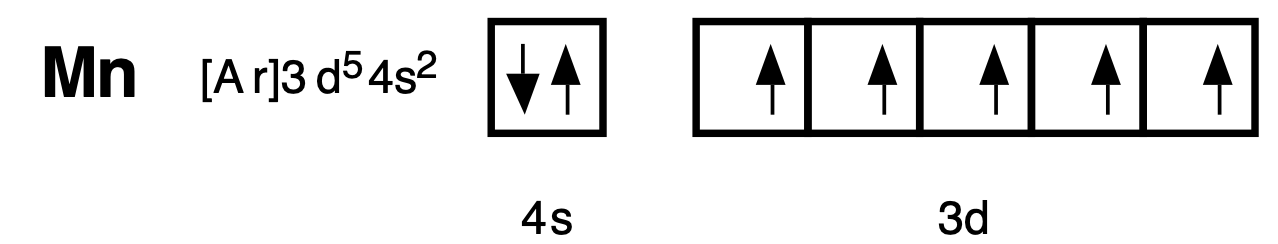
\includegraphics[width=0.5\columnwidth]{Bilder/mangan.png}
\end{center}

\begin{tabular}{cl}
    $\cvt{\blacksquare}$: & Die ersten 18 $e^-$ sind wie im Argon [Ar] angeordnet \\
    $\cgn{\blacksquare}$: & Hauptquantenzahl (Energieniveau), je höher die Zahl, desto weiter weg ist die Schale\\
    $\cbl{\blacksquare}$: & Bahndrehimpuls (Unterniveau), siehe \ref{chap:pauli} für die Anzahl der verfügbaren Boxen\\
    $\crd{\blacksquare}$: & Anzahl der $e^-$ im Unterniveau
\end{tabular}

\subsection{Formeln für Übungen}
Hinweis: Ergänzung zur Sektion 2.1.1 (Licht als Teilchen: Das Photon)

\renewcommand{\arraystretch}{1.9}
\resizebox{\columnwidth}{!}{%
\begin{tabular}{lcl}
    Mittlere opt. Leistung & $\bar{P} = \nu_{rep} \cdot E$ & [W] ($\nu_{rep}$ Freq. in [Hz], $E$ in [J]) \\ 
    Laser-Effizienz & $\eta = \frac{\bar{P}}{P_{ext}}$ & [dimensionslos] o. [\%] \\ 
    Spitzenleistung & $P_{max} = \frac{E}{\tau}$ & [W] ($\tau$ Impulsdauer in [s]) \\ 
    Max. Intensität (fokuss.) & $I_{max} = \frac{P_{max}}{\pi \lambda^2}$ & [W/m$^2$] (Fokus mit Radius $\lambda$) \\ 
    Photonenenergie & $E_{phot} = h\nu = \frac{hc}{\lambda}$ & [J] oder [eV] \\ 
    \textbf{Emittierte Photonen/s} & $n_{phot} = \frac{P}{E_{phot}}$ & [s$^{-1}$] \\ 
    \textbf{Erzeugter Strom} & $I = n_{phot} \cdot \eta \cdot e$ & [A]\\
    Umlaufzeit Resonator & $t = \frac{2l}{c}$ & [s] ($l$ = Resonatorlänge [m]) \\ 
    Resonatorenergie & $E_{Kav} = P_{Kav} \cdot t$ & [J] \\ 
    Gespeicherte Photonen & $N_{Kav} = \frac{E_{Kav}}{E_{phot}}$ & [dimensionslos] \\ 
\end{tabular}%
}
\newline
\newline
\textbf{Gruppe 3: Photoelektrischer Effekt}

\resizebox{\columnwidth}{!}{%
\begin{tabular}{lcl}
    Austrittsarbeit & $\Phi = \frac{hc}{\lambda_{max}}$ & [J] oder [eV] \\ 
    Photonenfluss & $\Gamma_{ph} = \frac{I_{light}}{E_{ph}}$ & [m$^{-2}$s$^{-1}$] ($I_{light}$ in [W/m$^2$]) \\ 
    Max. Photostromdichte & $J = e \cdot \Gamma_{ph} = \frac{e \cdot I_{light}}{E_{ph}}$ & [A/m$^2$] ($e$ Elementarladung) \\ 
\end{tabular}%
}
\newline
\newline

\textbf{Gruppe 4: Welle-Teilchen-Dualismus (de Broglie)}

Hinweis: Ergänzung zur Sektion 2.1.3 (Elektron als Welle: de Broglie Wellenlänge),

\resizebox{\columnwidth}{!}{%
\begin{tabular}{lcl}
    De-Broglie-Wellenlänge ($v$ bekannt) & $\lambda = \frac{h}{m \cdot v}$ & [m] \\ 
    De-Broglie-Wellenlänge ($U$ bekannt) & $\lambda = \frac{h}{\sqrt{2 \cdot m \cdot E_{kin}}} = \frac{h}{\sqrt{2 \cdot m \cdot e \cdot U}}$ & [m] ($U$ Spannung in [V]) \\ 
\end{tabular}%
}
\newline
\newline
\textbf{Gruppe 5: Quantenmechanik (Tunneleffekt)}

Hinweis: Ergänzung zur Sektion 2.2.1.2 (Potential mit Höhe V0 und Breite a: Tunnel-Effekt)

\resizebox{\columnwidth}{!}{%
\begin{tabular}{lcl}
    Dämpfungsfaktor & $\alpha = \frac{\sqrt{2 \cdot m \cdot (V_0 - E)}}{\hbar}$ & [m$^{-1}$] ($V_0$ und $E$ in [J]) \\ 
    Hilfskonstante $D$ & $D = \frac{V_0^2}{4 \cdot E \cdot (V_0 - E)}$ & [dimensionslos] \\ 
    Tunnelwahrscheinlichkeit & $T = \frac{1}{1 + D \cdot \sinh^2(\alpha \cdot a)}$ & [dimensionslos] ($a$ Barrierenbreite [m]) \\ 
    Definition $\sinh$ & $\sinh(\alpha \cdot a) = \frac{e^{\alpha \cdot a} - e^{-\alpha \cdot a}}{2}$ & Nützlich für exakte Berechnungen \\ 
\end{tabular}%
}
\renewcommand{\arraystretch}{1}